\documentclass[11pt]{article}

\usepackage[margin=0.85in]{geometry}
\usepackage[T1]{fontenc}
\usepackage{lmodern}
\usepackage{microtype}
\usepackage{xcolor}
\usepackage{booktabs}
\usepackage{longtable}
\usepackage{array}
\usepackage{enumitem}
\usepackage{hyperref}
\usepackage{listings}
\usepackage{tikz}
\usepackage{amsmath}
\usepackage{fancyhdr}
\usepackage{titlesec}
\usepackage{caption}
\usetikzlibrary{arrows.meta, positioning, shapes.geometric, shapes.misc, fit}

\hypersetup{
  colorlinks=true,
  linkcolor=blue!50!black,
  urlcolor=blue!50!black
}

\pagestyle{fancy}
\fancyhf{}
\lhead{\texttt{nr\_v2x\_ngsim\_deepc\_copy.cc} and MATLAB DeePC Guide}
\rhead{\thepage}

\definecolor{codebg}{RGB}{248,248,248}
\definecolor{commentgreen}{RGB}{0,110,70}
\definecolor{keywordblue}{RGB}{0,70,160}
\definecolor{stringred}{RGB}{150,35,35}
\definecolor{lightblue}{RGB}{235,244,255}
\definecolor{lightgreen}{RGB}{237,250,241}
\definecolor{lightyellow}{RGB}{255,249,224}
\definecolor{lightorange}{RGB}{255,242,226}
\definecolor{lightred}{RGB}{255,235,235}
\definecolor{lightpurple}{RGB}{246,238,255}

\lstdefinestyle{cppstyle}{
  language=C++,
  backgroundcolor=\color{codebg},
  basicstyle=\ttfamily\small,
  keywordstyle=\color{keywordblue}\bfseries,
  commentstyle=\color{commentgreen},
  stringstyle=\color{stringred},
  numbers=left,
  numberstyle=\tiny\color{gray},
  stepnumber=1,
  numbersep=8pt,
  showstringspaces=false,
  breaklines=true,
  frame=single,
  rulecolor=\color{black!20},
  tabsize=4
}

\lstdefinestyle{matlabstyle}{
  language=Matlab,
  backgroundcolor=\color{codebg},
  basicstyle=\ttfamily\small,
  keywordstyle=\color{keywordblue}\bfseries,
  commentstyle=\color{commentgreen},
  stringstyle=\color{stringred},
  numbers=left,
  numberstyle=\tiny\color{gray},
  stepnumber=1,
  numbersep=8pt,
  showstringspaces=false,
  breaklines=true,
  frame=single,
  rulecolor=\color{black!20},
  tabsize=4
}

\lstdefinestyle{textstyle}{
  backgroundcolor=\color{codebg},
  basicstyle=\ttfamily\small,
  breaklines=true,
  frame=single,
  rulecolor=\color{black!20}
}

\titleformat{\section}{\Large\bfseries}{\thesection}{0.6em}{}
\titleformat{\subsection}{\large\bfseries}{\thesubsection}{0.6em}{}
\titleformat{\subsubsection}{\normalsize\bfseries}{\thesubsubsection}{0.6em}{}
\setlist[itemize]{leftmargin=1.3em}
\setlist[enumerate]{leftmargin=1.5em}
\newcolumntype{L}[1]{>{\raggedright\arraybackslash}p{#1}}
\DeclareRobustCommand{\code}[1]{\texttt{\detokenize{#1}}}
\pdfstringdefDisableCommands{%
  \def\code#1{#1}%
}

\title{
  Closed-Loop NR-V2X DeePC Simulation Guide\\
  \large Explanation of \texttt{scratch/nr\_v2x\_ngsim\_deepc\_copy.cc} and
  \texttt{matlab/matlab\_deepc\_file\_controller.m}
}
\author{}
\date{}

\begin{document}
\maketitle

\begin{abstract}
This document explains the current ns-3 NR-V2X simulation code and the MATLAB
DeePC file controller used with it.  The C++ program creates vehicle nodes from
NGSIM trajectories, configures NR sidelink communication, sends ETSI CAM
messages, computes KPI samples, and optionally exchanges JSON files with a
MATLAB/YALMIP DeePC controller.  The MATLAB program watches the bridge request
directory, solves a classical Hankel DeePC optimization, and writes control
commands back to ns-3.  The goal of this guide is to make the code readable to a
professor or reviewer by documenting constants, variables, data structures,
function inputs and outputs, and the full program flow.
\end{abstract}

\tableofcontents
\newpage

\section{Executive Summary}

\subsection{Research Purpose}

The simulation studies congestion control for NR-V2X sidelink CAM broadcasting.
Each simulated vehicle periodically sends Cooperative Awareness Messages (CAMs).
The controllable inputs are:

\begin{itemize}
  \item transmit power, measured in dBm;
  \item CAM beacon interval, measured in seconds.
\end{itemize}

The measured outputs used by DeePC are:

\begin{itemize}
  \item packet reception ratio, \code{prr_awareness};
  \item packet inter-reception time, \code{pir_s};
  \item channel busy ratio, \code{cbr}.
\end{itemize}

The C++ code can run in two modes:

\begin{enumerate}
  \item \textbf{Open-loop PRBS mode}: read \code{prbs_schedule.csv} and apply a
  precomputed sequence of transmit powers and beacon intervals.
  \item \textbf{Closed-loop DeePC bridge mode}: disable the PRBS input schedule,
  periodically write KPI history to JSON, wait for MATLAB to solve DeePC, then
  apply the returned control input.
\end{enumerate}

\subsection{Source Files}

\begin{center}
\begin{tabular}{L{0.34\linewidth}L{0.56\linewidth}}
\toprule
File & Role \\
\midrule
\code{scratch/nr_v2x_ngsim_deepc_copy.cc} &
Main ns-3 C++ simulation.  Loads mobility and inputs, creates vehicles, configures
NR-V2X sidelink, installs CAM applications, logs KPIs, and optionally runs the
file-based DeePC bridge. \\
\code{matlab/matlab_deepc_file_controller.m} &
MATLAB/YALMIP controller.  Reads ns-3 bridge requests, solves a classical Hankel
DeePC quadratic program, and writes response JSON files containing the next
transmit power and beacon interval. \\
\code{data/processed/ngsim_us101_10min_0p1s.csv} &
Default processed mobility input.  One row is one vehicle position sample. \\
\code{data/processed/prbs_schedule.csv} &
Default open-loop input schedule.  One row is one time-varying command. \\
\code{data/output/deepc_open_loop_250veh/matlab_deepc_data.mat} &
Default MATLAB DeePC data file containing Hankel matrices, normalization
statistics, and horizon information. \\
\bottomrule
\end{tabular}
\end{center}

\section{System-Level Block Diagram}

\begin{center}
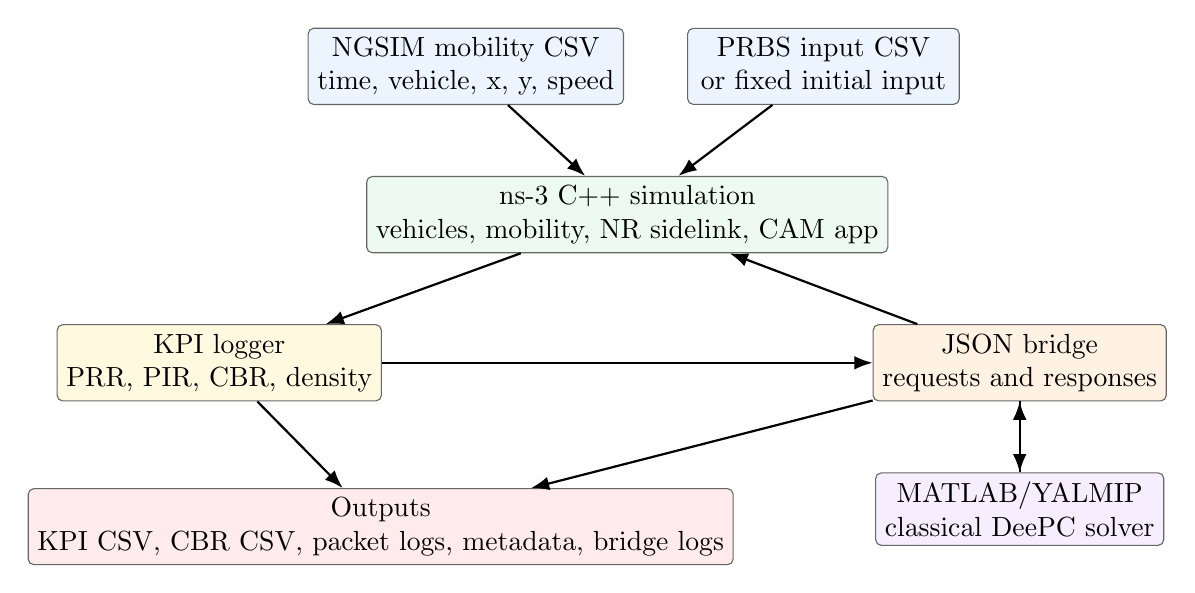
\begin{tikzpicture}[
  box/.style={rectangle, draw=black!60, rounded corners=2pt, align=center,
              minimum width=3.45cm, minimum height=0.82cm},
  wide/.style={rectangle, draw=black!60, rounded corners=2pt, align=center,
               minimum width=5.1cm, minimum height=0.82cm},
  arrow/.style={-Latex, thick},
  node distance=0.75cm
]
\node[box, fill=lightblue] (mob) {NGSIM mobility CSV\\time, vehicle, x, y, speed};
\node[box, fill=lightblue, right=0.8cm of mob] (input) {PRBS input CSV\\or fixed initial input};
\node[wide, fill=lightgreen, below=0.9cm of mob, xshift=2.05cm] (ns3) {ns-3 C++ simulation\\vehicles, mobility, NR sidelink, CAM app};
\node[box, fill=lightyellow, below left=0.9cm and -0.2cm of ns3] (kpi) {KPI logger\\PRR, PIR, CBR, density};
\node[box, fill=lightorange, below right=0.9cm and -0.2cm of ns3] (bridge) {JSON bridge\\requests and responses};
\node[box, fill=lightpurple, below=0.9cm of bridge] (matlab) {MATLAB/YALMIP\\classical DeePC solver};
\node[wide, fill=lightred, below=1.1cm of kpi, xshift=2.05cm] (out) {Outputs\\KPI CSV, CBR CSV, packet logs, metadata, bridge logs};

\draw[arrow] (mob) -- (ns3);
\draw[arrow] (input) -- (ns3);
\draw[arrow] (ns3) -- (kpi);
\draw[arrow] (kpi) -- (out);
\draw[arrow] (kpi) -- (bridge);
\draw[arrow] (bridge) -- (matlab);
\draw[arrow] (matlab) -- (bridge);
\draw[arrow] (bridge) -- (ns3);
\draw[arrow] (bridge) -- (out);
\end{tikzpicture}
\end{center}

\section{Constants, Parameters, and Global State}

This section is intentionally early in the document because these values define
the experiment before the functions are discussed.

\subsection{Compile-Time Constants}

\begin{center}
\begin{tabular}{L{0.28\linewidth}L{0.18\linewidth}L{0.44\linewidth}}
\toprule
Constant & Value & Meaning \\
\midrule
\code{kPi} & \code{3.14159265358979323846} &
Mathematical pi used for heading and longitude calculations. \\
\code{kDotOneMicro} & \code{1e7} &
Scale factor used by ETSI CAM latitude/longitude fields.  A degree value is
multiplied by 10,000,000. \\
\code{kLocalOriginLatitudeDeg} & \code{37.0} &
Local latitude origin used to convert NGSIM local meters into approximate
geographic latitude. \\
\code{kLocalOriginLongitudeDeg} & \code{-122.0} &
Local longitude origin used to convert NGSIM local meters into approximate
geographic longitude. \\
\bottomrule
\end{tabular}
\end{center}

\subsection{Default Experiment Parameters in \code{main()}}

\begin{center}
\begin{longtable}{L{0.28\linewidth}L{0.18\linewidth}L{0.44\linewidth}}
\toprule
Parameter & Default & Meaning \\
\midrule
\endhead
\code{mobilityCsv} & \code{data/processed/ngsim_us101_10min_0p1s.csv} &
Processed NGSIM mobility data. \\
\code{inputCsv} & \code{data/processed/prbs_schedule.csv} &
Open-loop PRBS control schedule. \\
\code{kpiCsv} & \code{data/output/kpi_timeseries_deepc_copy_run01.csv} &
Main KPI time-series output. \\
\code{cbrCsv} & \code{data/output/cbr_timeseries_deepc_copy_run01.csv} &
Standalone CBR output written by \code{CbrLogger}. \\
\code{simTimeSeconds} & \code{300.0} &
Total simulation time. \\
\code{warmupS} & \code{10.0} &
Initial time excluded from KPI evaluation. \\
\code{cooldownS} & \code{10.0} &
Final time excluded from KPI evaluation. \\
\code{seed}, \code{run} & \code{12345}, \code{1} &
ns-3 RNG seed and run number. \\
\code{useIPv6} & \code{false} &
IPv6 flag.  The current merged file supports IPv4 only and aborts if IPv6 is
requested. \\
\code{maxCamSizeBytes} & \code{300} &
Maximum encoded CAM packet size setting passed to each CAM application. \\
\code{port} & \code{8000} &
UDP port used by all CAM applications. \\
\code{useInputSchedule} & \code{true} &
If true, scheduled PRBS inputs are applied.  If false, fixed or DeePC bridge
inputs are used. \\
\code{etsiCamGeneration} & \code{true} &
If true, the CAM service uses ETSI-style decentralized triggering.  If false,
the code forces fixed periodic CAM generation at \code{T_GenCamMax}. \\
\code{fixedBeaconIntervalS} & \code{0.1} &
Initial or fixed beacon interval. \\
\code{slBearersActivationTime} & \code{2.0 s} &
Time when sidelink transmit and receive bearers are activated. \\
\code{camApplicationStartDelay} & \code{200 ms} &
Extra delay after bearer activation before CAM applications can start. \\
\code{harqEnabled} & \code{true} &
Enables HARQ in sidelink bearer configuration. \\
\code{delayBudget} & \code{0 s} &
Packet delay budget passed into the sidelink bearer information. \\
\code{centralFrequencyBandSl} & \code{5.9e9 Hz} &
Sidelink carrier frequency. \\
\code{bandwidthBandSl} & \code{100} &
Bandwidth in 100 kHz units, so 100 means 10 MHz. \\
\code{txPower} & \code{20.0 dBm} &
Initial transmit power before schedule or DeePC updates. \\
\code{tddPattern} & \code{DL|DL|DL|F|UL|UL|UL|UL|UL|UL|} &
TDD pattern used by the sidelink preconfiguration. \\
\code{slBitMap} & \code{1|1|1|1|1|1|0|0|0|1|1|1} &
Sidelink time-resource bitmap parsed by \code{GetSlBitmapFromString()}. \\
\code{numerologyBwpSl} & \code{0} &
NR numerology for the sidelink bandwidth part. \\
\code{enableSensing} & \code{true} &
Experiment requires sensing-based sidelink resource selection because CBR is
derived from sensing/PHY traces.  The program aborts if this is false. \\
\code{slSensingWindow} & \code{100 ms} &
Sidelink sensing window. \\
\code{slSelectionWindow} & \code{5 slots} &
Sidelink resource selection window. \\
\code{slSubchannelSize} & \code{50} &
Subchannel size used by the sidelink resource pool factory. \\
\code{slMaxNumPerReserve} & \code{3} &
Maximum number of reserved resources per reservation period. \\
\code{slProbResourceKeep} & \code{0.0} &
Probability of keeping a previously selected sidelink resource. \\
\code{slMaxTxTransNumPssch} & \code{5} &
Maximum number of PSSCH transmissions configured in the sidelink preconfiguration. \\
\code{reservationPeriod} & \code{100 ms} &
Resource reservation interval. \\
\code{t1}, \code{t2} & \code{2}, \code{33} &
Sensing-based selection timing parameters. \\
\code{slThresPsschRsrp} & \code{-128 dBm} &
PSSCH-RSRP threshold used by sidelink sensing. \\
\code{enableChannelRandomness} & \code{true} &
Controls whether the ThreeGPP channel update period is randomized over time. \\
\code{channelUpdatePeriod} & \code{500 ms} &
Channel update period used when channel randomness is enabled. \\
\code{mcs} & \code{6} &
Fixed sidelink MCS. \\
\code{awarenessRangeM} & \code{300.0 m} &
Distance threshold used in the PRR denominator and numerator. \\
\code{kpiWindowS} & \code{1.0 s} &
Sliding window over which PRR and PIR are computed.  The program currently
aborts unless this is exactly 1.0 s. \\
\code{sampleTimeS} & \code{1} &
KPI sampling interval in seconds.  Note: the inline code comment says 100 ms,
but the current numeric value is 1 s. \\
\code{maxVehicles} & \code{0} &
Maximum number of vehicles to simulate.  Zero means all loaded vehicles. \\
\code{enableCoreFilter} & \code{true} &
If true, KPIs are measured only inside a central road corridor region. \\
\code{coreAxis} & \code{auto} &
Longitudinal axis for the core filter.  Auto chooses the axis with larger span. \\
\code{coreGuardBandM} & \code{120.0 m} &
Distance removed from each end of the study corridor when deriving the core. \\
\code{coreMin}, \code{coreMax} & \code{NaN}, \code{NaN} &
Optional manual core bounds.  If left as NaN, the program derives them from the
study bounds and guard band. \\
\code{requireFullDataCoverage} & \code{true} &
If true, aborts when mobility or input schedule does not cover the requested
simulation/evaluation interval. \\
\code{validateOnly} & \code{false} &
If true, validates data and exits before building NR devices. \\
\code{allowProtectedOutput} & \code{false} &
Protects important DeePC data paths from accidental overwrite. \\
\code{enableDeepcBridge} & \code{false} &
Enables closed-loop file-based DeePC control.  This must be used with
\code{useInputSchedule=false}. \\
\code{deepcBridgeDir} & \code{data/output/deepc_matlab_bridge_run01/bridge} &
Directory containing bridge request and response JSON files. \\
\code{deepcControlIntervalS} & \code{0.1 s} &
How often the bridge checks for a new KPI sample and possibly asks MATLAB for a
new control. \\
\code{deepcPastHorizon} & \code{20} &
Number of past KPI samples sent to the DeePC controller. \\
\code{deepcFutureHorizon} & \code{10} &
Number of future steps optimized by the DeePC controller. \\
\code{deepcResponseTimeoutS} & \code{30.0 s} &
Wall-clock timeout while ns-3 waits for MATLAB to write a response JSON file. \\
\bottomrule
\end{longtable}
\end{center}

\subsection{Global Maps and Their Meaning}

\begin{center}
\begin{longtable}{L{0.34\linewidth}L{0.56\linewidth}}
\toprule
Global variable & Purpose \\
\midrule
\endhead
\code{g_mobilityByVehicle} &
Maps original NGSIM vehicle ID to all \code{MobilityRow} records for that
vehicle.  It is populated by \code{LoadMobilityCsv()}. \\
\code{g_inputSchedule} &
Vector of \code{InputCommand} records read from the PRBS input CSV. \\
\code{g_vehicleIdToNodeId} &
Maps NGSIM vehicle IDs to ns-3 node IDs after node creation. \\
\code{g_nodeIdToVehicleId} &
Reverse map from ns-3 node ID to original NGSIM vehicle ID. \\
\code{g_nodeIdToNode} &
Maps ns-3 node IDs to actual \code{Ptr<Node>} handles.  Used by receive logging
and CBR filtering. \\
\code{g_nodeIdToActiveTimeRangeS} &
Maps ns-3 node IDs to the first and last mobility timestamp available for that
vehicle.  This prevents inactive vehicles from contributing to KPIs. \\
\code{g_apps} &
Maps ns-3 node IDs to installed \code{CamApplication} objects so the code can
change every vehicle's beacon interval at runtime. \\
\bottomrule
\end{longtable}
\end{center}

\section{Data Structures}

\subsection{C++ Structures}

\begin{center}
\begin{longtable}{L{0.21\linewidth}L{0.30\linewidth}L{0.39\linewidth}}
\toprule
Structure & Fields & Meaning \\
\midrule
\endhead
\code{MobilityRow} &
\code{timeS}, \code{vehicleId}, \code{xM}, \code{yM}, \code{vxMps},
\code{vyMps}, \code{speedMps}, \code{laneId} &
One row from the mobility CSV.  It represents one vehicle's position and
velocity at one timestamp. \\
\code{InputCommand} &
\code{timeS}, \code{txPowerDbm}, \code{beaconIntervalS} &
One control command.  In PRBS mode it comes from the input CSV.  In DeePC mode it
comes from the MATLAB response. \\
\code{TxEvent} &
\code{timeS}, \code{txNodeId}, \code{seq}, \code{posTx},
\code{eligibleRxCount}, \code{eligibleRxCountsByBin},
\code{rxDistanceAtTxM} &
One transmitted CAM.  It stores the transmitter position and all receivers that
were eligible at transmit time. \\
\code{RxEvent} &
\code{timeS}, \code{txNodeId}, \code{rxNodeId}, \code{seq}, \code{posTx},
\code{posRx}, \code{distanceAtTxM}, \code{distanceAtRxM}, \code{pirS},
\code{delayS} &
One successfully received CAM.  It links back to a \code{TxEvent} by
\code{txNodeId} and \code{seq}. \\
\code{KpiSample} &
\code{timeS}, current input values, traffic context, \code{prrAwareness},
\code{pirS}, \code{cbr}, \code{sensingExclusionRatio} &
One row of the main KPI time series.  The DeePC bridge stores a deque of these
samples and sends the latest history to MATLAB. \\
\bottomrule
\end{longtable}
\end{center}

\subsection{Example Data Instances}

\begin{lstlisting}[style=textstyle, caption={Example mobility and input records.}]
MobilityRow{
  timeS = 12.4,
  vehicleId = 104,
  xM = 23.7,
  yM = 818.2,
  vxMps = 0.4,
  vyMps = 18.6,
  speedMps = 18.7,
  laneId = 3
}

InputCommand{
  timeS = 5.0,
  txPowerDbm = 23.0,
  beaconIntervalS = 0.2
}
\end{lstlisting}

\begin{lstlisting}[style=textstyle, caption={Example packet events used for PRR and PIR.}]
TxEvent{
  timeS = 12.300,
  txNodeId = 7,
  seq = 42,
  posTx = Vector(100, 500, 0),
  eligibleRxCount = 2,
  eligibleRxCountsByBin = [1, 0, 0, 0, 1],
  rxDistanceAtTxM = {8: 20.0, 9: 280.0, 10: 350.0}
}

RxEvent{
  timeS = 12.305,
  txNodeId = 7,
  rxNodeId = 9,
  seq = 42,
  posTx = Vector(100, 500, 0),
  posRx = Vector(380, 500, 0),
  distanceAtTxM = 280.0,
  distanceAtRxM = 279.5,
  pirS = 0.3,
  delayS = 0.005
}
\end{lstlisting}

\subsection{Bridge JSON Schema}

When closed-loop bridge mode is enabled, ns-3 writes a JSON request.  The most
important arrays are:

\begin{center}
\begin{tabular}{L{0.24\linewidth}L{0.20\linewidth}L{0.46\linewidth}}
\toprule
JSON field & Length & Meaning \\
\midrule
\code{previous_u} & \code{2} &
Last applied input: \code{[tx_power_dbm, beacon_interval_s]}. \\
\code{u_ini} & \code{2 * past_horizon} &
Past input trajectory. \\
\code{y_ini} & \code{3 * past_horizon} &
Past output trajectory: \code{prr_awareness}, \code{pir_s}, \code{cbr}. \\
\code{d_ini} & \code{5 * past_horizon} &
Past context trajectory: active count, density, 150 m neighbors, 300 m
neighbors, sensing exclusion ratio. \\
\code{d_future} & \code{5 * future_horizon} &
Future context assumption.  The current C++ bridge repeats the latest measured
context for all future steps. \\
\bottomrule
\end{tabular}
\end{center}

MATLAB writes a matching response:

\begin{lstlisting}[style=textstyle, caption={Example DeePC response JSON.}]
{
  "step": 4,
  "time_s": 11.4,
  "success": true,
  "tx_power_dbm": 17.25,
  "beacon_interval_s": 0.12,
  "objective": 8.91,
  "solve_time_s": 0.035,
  "solver_status": "Successfully solved",
  "controller": "matlab_yalmip_classical_deepc"
}
\end{lstlisting}

\section{C++ Program Flow}

\subsection{\code{main(argc, argv)} Input and Output}

\begin{center}
\begin{tabular}{L{0.24\linewidth}L{0.66\linewidth}}
\toprule
Item & Explanation \\
\midrule
Input &
\code{argc} and \code{argv} from the command line.  ns-3 \code{CommandLine}
parses these into simulation parameters such as \code{--simTime},
\code{--maxVehicles}, \code{--enableDeepcBridge}, and output paths. \\
Output &
Returns \code{0} on successful completion.  Side effects are the important
outputs: CSV logs, JSON metadata, optional bridge request/response files, and
console status messages. \\
Major state changed &
Fills global mobility/input maps, creates ns-3 nodes and devices, installs
applications, schedules simulator events, and runs/destroys the simulator. \\
\bottomrule
\end{tabular}
\end{center}

\subsection{High-Level Flow of \code{main()}}

\begin{center}
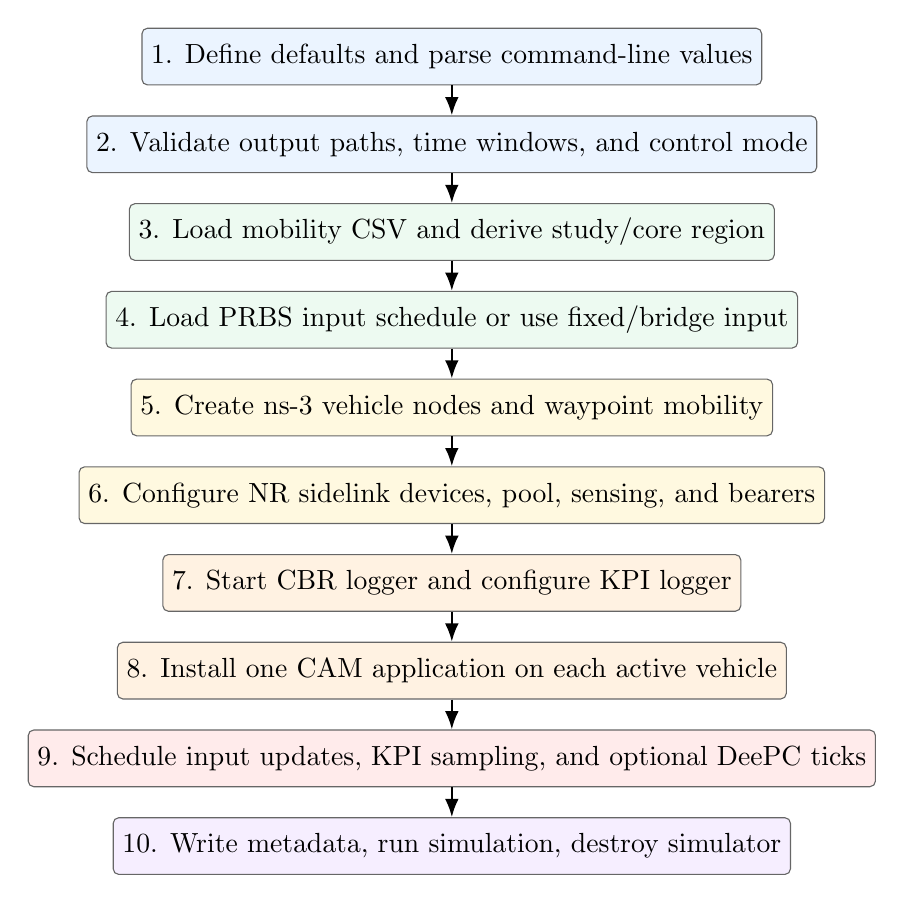
\begin{tikzpicture}[
  box/.style={rectangle, draw=black!60, rounded corners=2pt, align=center,
              minimum width=5.8cm, minimum height=0.72cm},
  arrow/.style={-Latex, thick},
  node distance=0.38cm
]
\node[box, fill=lightblue] (p) {1. Define defaults and parse command-line values};
\node[box, fill=lightblue, below=of p] (v) {2. Validate output paths, time windows, and control mode};
\node[box, fill=lightgreen, below=of v] (m) {3. Load mobility CSV and derive study/core region};
\node[box, fill=lightgreen, below=of m] (i) {4. Load PRBS input schedule or use fixed/bridge input};
\node[box, fill=lightyellow, below=of i] (n) {5. Create ns-3 vehicle nodes and waypoint mobility};
\node[box, fill=lightyellow, below=of n] (r) {6. Configure NR sidelink devices, pool, sensing, and bearers};
\node[box, fill=lightorange, below=of r] (k) {7. Start CBR logger and configure KPI logger};
\node[box, fill=lightorange, below=of k] (a) {8. Install one CAM application on each active vehicle};
\node[box, fill=lightred, below=of a] (s) {9. Schedule input updates, KPI sampling, and optional DeePC ticks};
\node[box, fill=lightpurple, below=of s] (run) {10. Write metadata, run simulation, destroy simulator};
\draw[arrow] (p) -- (v);
\draw[arrow] (v) -- (m);
\draw[arrow] (m) -- (i);
\draw[arrow] (i) -- (n);
\draw[arrow] (n) -- (r);
\draw[arrow] (r) -- (k);
\draw[arrow] (k) -- (a);
\draw[arrow] (a) -- (s);
\draw[arrow] (s) -- (run);
\end{tikzpicture}
\end{center}

\subsection{Packet and KPI Flow}

\begin{center}
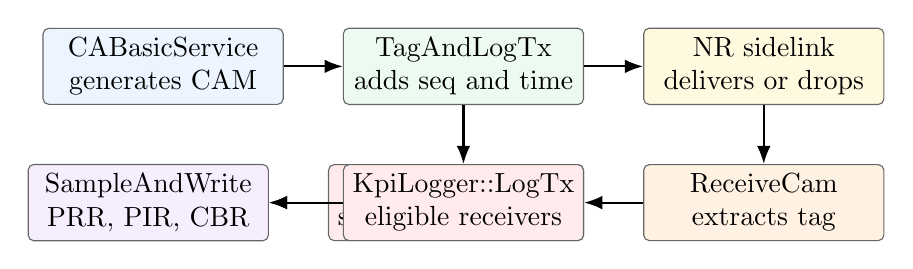
\begin{tikzpicture}[
  box/.style={rectangle, draw=black!60, rounded corners=2pt, align=center,
              minimum width=3.05cm, minimum height=0.78cm},
  arrow/.style={-Latex, thick},
  node distance=0.75cm
]
\node[box, fill=lightblue] (cam) {CABasicService\\generates CAM};
\node[box, fill=lightgreen, right=of cam] (tag) {TagAndLogTx\\adds seq and time};
\node[box, fill=lightyellow, right=of tag] (radio) {NR sidelink\\delivers or drops};
\node[box, fill=lightorange, below=of radio] (rx) {ReceiveCam\\extracts tag};
\node[box, fill=lightred, left=of rx] (logrx) {KpiLogger::LogRx\\successful reception};
\node[box, fill=lightpurple, left=of logrx] (sample) {SampleAndWrite\\PRR, PIR, CBR};
\node[box, fill=lightred, below=of tag] (logtx) {KpiLogger::LogTx\\eligible receivers};
\draw[arrow] (cam) -- (tag);
\draw[arrow] (tag) -- (radio);
\draw[arrow] (tag) -- (logtx);
\draw[arrow] (radio) -- (rx);
\draw[arrow] (rx) -- (logrx);
\draw[arrow] (logtx) -- (sample);
\draw[arrow] (logrx) -- (sample);
\end{tikzpicture}
\end{center}

\section{C++ Helper Functions}

\subsection{Geometry, Time Coverage, and Core Region}

\begin{center}
\begin{longtable}{L{0.24\linewidth}L{0.27\linewidth}L{0.18\linewidth}L{0.21\linewidth}}
\toprule
Function & Inputs & Output & What it does \\
\midrule
\endhead
\code{Distance2d(a,b)} &
Two ns-3 \code{Vector} values. &
\code{double} distance in meters. &
Computes planar Euclidean distance using x and y only. \\
\code{ClampToLong(value,min,max)} &
Floating value and integer bounds. &
\code{long}. &
Clamps then rounds a value so CAM fields stay inside valid ETSI numeric ranges. \\
\code{EncodeLatitudeFromLocalY(yM)} &
Local y coordinate in meters. &
Encoded latitude integer. &
Converts local y meters to approximate latitude and scales by \code{1e7}. \\
\code{EncodeLongitudeFromLocalX(xM)} &
Local x coordinate in meters. &
Encoded longitude integer. &
Converts local x meters to approximate longitude, correcting meters per degree by
origin latitude. \\
\code{IsInsideCoreRegion(coordinate,coreMin,coreMax)} &
One coordinate and core bounds. &
\code{bool}. &
Returns true when the coordinate lies inside the evaluation corridor. \\
\code{IsNodeActiveAtTime(nodeId,timeS)} &
Node ID and simulation time. &
\code{bool}. &
Checks whether that vehicle has mobility data at the requested time. \\
\code{ComputeMobilityTimeRange(rows)} &
Vector of \code{MobilityRow}. &
\code{pair<min,max>}. &
Finds the first and last mobility timestamps for one vehicle. \\
\code{ComputeMobilityTimeRangeForVehicles(vehicleIds)} &
Selected original vehicle IDs. &
\code{pair<min,max>}. &
Finds total time coverage across the selected vehicles. \\
\code{ComputeInputScheduleTimeRange()} &
No explicit input; uses \code{g_inputSchedule}. &
\code{pair<min,max>}. &
Finds first and last command times in the input schedule. \\
\code{ValidateTenMinuteDataCoverage(...)} &
Simulation time, evaluation window, schedule flag, coverage flag, selected vehicles. &
No return; aborts on invalid coverage. &
Ensures mobility covers the KPI evaluation interval and, if enabled, input
schedule covers the whole simulation. \\
\code{ComputeStudyBounds(axis)} &
\code{"x"} or \code{"y"}. &
\code{pair<min,max>}. &
Scans all mobility rows and returns the spatial study extent along one axis. \\
\code{ResolveCoreAxis(requestedAxis)} &
\code{"auto"}, \code{"x"}, or \code{"y"}. &
Resolved axis string. &
If auto, chooses the larger of the x-span and y-span as the longitudinal road
axis. \\
\code{GetCoreCoordinate(position,axis)} &
Position and resolved axis. &
\code{double}. &
Returns either \code{position.x} or \code{position.y} for core filtering. \\
\bottomrule
\end{longtable}
\end{center}

\subsection{File Loading and Mobility Installation}

\begin{center}
\begin{longtable}{L{0.24\linewidth}L{0.27\linewidth}L{0.18\linewidth}L{0.21\linewidth}}
\toprule
Function & Inputs & Output & What it does \\
\midrule
\endhead
\code{LoadMobilityCsv(path)} &
Path to processed mobility CSV. &
No return; fills \code{g_mobilityByVehicle}. &
Reads each CSV row, converts text to numeric fields, creates a \code{MobilityRow},
and appends it to that vehicle's row vector. \\
\code{LoadInputScheduleCsv(path)} &
Path to input schedule CSV. &
No return; fills \code{g_inputSchedule}. &
Reads \code{time_s}, \code{tx_power_dbm}, and \code{beacon_interval_s} into
\code{InputCommand} records. \\
\code{InstallWaypointMobility(node,rows)} &
An ns-3 node and its mobility rows. &
No return; modifies node. &
Creates a \code{WaypointMobilityModel}, aggregates it to the node, and adds one
waypoint for each mobility row. \\
\code{GetSlBitmapFromString(slBitMapString,slBitMapVector)} &
String such as \code{1|1|0|1} and output vector. &
No return; fills vector. &
Splits the bitmap string and converts each token into a one-bit value for
sidelink time resources. \\
\bottomrule
\end{longtable}
\end{center}

\subsection{Runtime Input and Output Utilities}

\begin{center}
\begin{longtable}{L{0.24\linewidth}L{0.27\linewidth}L{0.18\linewidth}L{0.21\linewidth}}
\toprule
Function & Inputs & Output & What it does \\
\midrule
\endhead
\code{ApplyTxPowerToAllUes(ueDevs,pDbm)} &
UE net devices and power value. &
No return; changes PHY state. &
Iterates through every NR UE net device and every BWP, then calls
\code{SetTxPower(pDbm)} on each UE PHY. \\
\code{ApplyInputsAtTime(logger,ueDevs,pDbm,tbS)} &
KPI logger, devices, transmit power, beacon interval. &
No return; changes inputs. &
Updates current KPI input values, updates every CAM app's beacon interval, and
applies transmit power to every UE. \\
\code{ScheduleInputUpdates(logger,ueDevs)} &
KPI logger and UE devices. &
No return; schedules events. &
For each \code{InputCommand}, schedules \code{ApplyInputsAtTime()} at
\code{command.timeS}. \\
\code{ConnectCbrTraces(cbrLogger)} &
Pointer to \code{CbrLogger}. &
No return. &
Connects ns-3 trace sources for sensing algorithm diagnostics and PHY
channel-occupied events. \\
\code{DeriveSidecarPath(csvPath,suffix)} &
CSV path and suffix. &
Derived path string. &
Replaces \code{.csv} with a suffix, for example metadata or packet log names. \\
\code{StartsWithPathPrefix(path,prefix)} &
Two strings. &
\code{bool}. &
Small helper for protected output path checks. \\
\code{IsProtectedDeepcOutputPath(path)} &
Path string. &
\code{bool}. &
Returns true for important baseline DeePC output paths that should not be
overwritten by accident. \\
\code{ValidateSafeOutputPaths(kpiCsv,cbrCsv,allowProtectedOutput)} &
Output paths and override flag. &
No return; aborts on unsafe paths. &
Ensures KPI and CBR outputs differ and protects important existing DeePC data
unless explicitly allowed. \\
\code{JsonEscape(value)} &
String. &
Escaped string. &
Escapes characters before writing JSON manually from C++. \\
\code{WriteJsonArray(os,values)} &
Output stream and vector of doubles. &
No return; writes to stream. &
Writes a numeric JSON array. \\
\code{ExtractJsonNumber(content,key,value)} &
JSON text, key, output double. &
\code{bool}. &
Lightweight parser that extracts one numeric field from a response JSON file. \\
\code{ExtractJsonBool(content,key,value)} &
JSON text, key, output bool. &
\code{bool}. &
Lightweight parser that extracts one boolean field from a response JSON file. \\
\code{WriteMetadataJson(...)} &
Output paths, simulation parameters, radio parameters, and experiment settings. &
No return; writes JSON. &
Creates a metadata sidecar describing the dataset, KPI definitions, radio
settings, CAM generation rule, and DeePC dataset columns. \\
\bottomrule
\end{longtable}
\end{center}

\section{C++ Classes}

\subsection{\code{KpiPacketTag}}

\code{KpiPacketTag} is an ns-3 packet tag attached to each transmitted CAM.  It
is invisible to the application payload but travels with the packet inside the
simulation.

\begin{center}
\begin{tabular}{L{0.28\linewidth}L{0.22\linewidth}L{0.40\linewidth}}
\toprule
Method & Input/Output & Explanation \\
\midrule
\code{GetTypeId()} &
Returns ns-3 \code{TypeId}. &
Registers the tag type with ns-3. \\
\code{GetInstanceTypeId()} &
Returns ns-3 \code{TypeId}. &
Runtime type information for this tag instance. \\
\code{GetSerializedSize()} &
Returns \code{16}. &
The tag stores two 64-bit values. \\
\code{Serialize(i)} &
Writes to \code{TagBuffer}. &
Stores sequence number and transmit timestamp. \\
\code{Deserialize(i)} &
Reads from \code{TagBuffer}. &
Restores sequence number and transmit timestamp. \\
\code{Print(os)} &
Writes human-readable tag. &
Useful for debug printing. \\
\code{SetSequence()}, \code{GetSequence()} &
Set/get \code{uint64_t}. &
Packet sequence number local to a CAM application. \\
\code{SetTxTimeNs()}, \code{GetTxTimeNs()} &
Set/get nanoseconds. &
Transmit timestamp used to compute delay. \\
\bottomrule
\end{tabular}
\end{center}

\subsection{\code{KpiLogger}}

\code{KpiLogger} is the central measurement object.  It records packet
transmission opportunities, successful receptions, traffic context, CBR, and the
latest sample used by the DeePC bridge.

\subsubsection{Important Member Variables}

\begin{center}
\begin{longtable}{L{0.30\linewidth}L{0.60\linewidth}}
\toprule
Member variable & Meaning \\
\midrule
\endhead
\code{m_awarenessRangeM} &
PRR awareness distance.  A receiver inside this TX-time distance contributes to
the PRR opportunity count. \\
\code{m_kpiWindowS}, \code{m_sampleTimeS} &
Sliding KPI window length and output sampling interval. \\
\code{m_evalStartS}, \code{m_evalEndS} &
Warmup/cooldown evaluation limits. \\
\code{m_enableCoreFilter}, \code{m_coreAxis}, \code{m_coreMin}, \code{m_coreMax} &
Spatial core-region filter settings. \\
\code{m_densityLengthM} &
Road length used to convert active vehicle count into vehicles per km. \\
\code{m_cbrLogger} &
Pointer to the external CBR logger used to compute CBR and sensing exclusion
ratio at sample time. \\
\code{m_currentP}, \code{m_currentTb} &
Current transmit power and beacon interval.  These values are written into KPI
rows and bridge samples. \\
\code{m_latestSample}, \code{m_hasLatestSample} &
Most recent KPI sample and flag indicating whether it is valid. \\
\code{m_distanceBinEdgesM} &
Distance-bin edges for TX packet log columns: 0, 50, 100, 150, 200, 300 m. \\
\code{m_nodes}, \code{m_nodeIds} &
Evaluated ns-3 nodes and their IDs. \\
\code{m_ipToNodeId} &
IPv4-to-node map used to identify the transmitter in receive callbacks. \\
\code{m_txEvents}, \code{m_rxEvents} &
Sliding-window deques of recent transmissions and receptions. \\
\code{m_loggedRxTriples} &
Set of unique \((tx,rx,seq)\) triples already logged, used to remove duplicates. \\
\code{m_lastRxTimePerPair} &
Last successful receive time for each transmitter-receiver pair, used for PIR. \\
\code{m_out}, \code{m_txOut}, \code{m_rxOut} &
Main KPI, TX packet, and RX packet output streams. \\
\bottomrule
\end{longtable}
\end{center}

\subsubsection{Public Methods}

\begin{center}
\begin{longtable}{L{0.25\linewidth}L{0.27\linewidth}L{0.38\linewidth}}
\toprule
Method & Inputs and outputs & Function behavior \\
\midrule
\endhead
\code{Configure(...)} &
Inputs: node container, \code{CbrLogger}, output path, PRR range, window sizes,
evaluation window, core filter settings.  Output: none. &
Stores configuration, copies evaluated nodes, opens the KPI CSV, TX packet log,
and RX packet log, and writes their headers. \\
\code{RegisterNodeIpv4(nodeId,addr)} &
Input: node ID and IPv4 address.  Output: none. &
Builds a map from source IPv4 address to transmitting node ID for received CAMs. \\
\code{ResolveNodeIdFromIpv4(addr)} &
Input: IPv4 address.  Output: node ID or max \code{uint32_t}. &
Converts the sender IP in a received packet callback into an ns-3 node ID. \\
\code{SetCurrentInputs(pDbm,tbS)} &
Input: current power and beacon interval.  Output: none. &
Stores the input values that will be written in future KPI rows. \\
\code{HasLatestSample()} &
No input.  Output: bool. &
Returns true after at least one KPI sample has been computed. \\
\code{GetLatestSample()} &
No input.  Output: \code{KpiSample}. &
Returns the most recent KPI sample for the DeePC bridge. \\
\code{LogTx(txNodeId,seq,tTx,posTx)} &
Input: transmitter node, sequence, transmit time, transmitter position.  Output:
none. &
Rejects out-of-window, inactive, or out-of-core transmissions.  Counts eligible
receivers within the awareness range and distance bins, stores a \code{TxEvent},
writes the TX packet log, and prunes old events. \\
\code{LogRx(txNodeId,rxNodeId,seq,tRx,posTx,posRx,delayS)} &
Input: transmitter, receiver, sequence, receive time, current positions, delay.
Output: none. &
Finds the matching \code{TxEvent}, removes duplicates, computes PIR for this
transmitter-receiver pair, stores a \code{RxEvent}, writes the RX packet log, and
prunes old events. \\
\code{SampleAndWrite()} &
No explicit input; uses simulator time and stored events.  Output: scheduled
next sample and one CSV row. &
Computes PRR, PIR mean, CBR, sensing exclusion ratio, active vehicle count,
density, and neighbor counts.  Updates \code{m_latestSample}, writes the KPI CSV,
and schedules itself again after \code{sampleTimeS}. \\
\bottomrule
\end{longtable}
\end{center}

\subsubsection{Private Methods}

\begin{center}
\begin{longtable}{L{0.25\linewidth}L{0.27\linewidth}L{0.38\linewidth}}
\toprule
Method & Inputs and outputs & Function behavior \\
\midrule
\endhead
\code{ComputeTrafficContext()} &
No input.  Output: \code{TrafficContext}. &
Collects active vehicles inside the core region at the current time, computes
density per km, and computes mean neighbor counts within 150 m and 300 m. \\
\code{PruneOldEvents()} &
No input.  Output: none. &
Removes TX/RX events older than the sliding KPI window and removes RX events
whose matching TX event has left the window. \\
\code{GetDistanceBinIndex(distanceM)} &
Input: distance.  Output: bin index or \code{-1}. &
Classifies a TX-time receiver distance into bins
\([0,50), [50,100), [100,150), [150,200), [200,300]\) meters. \\
\code{BuildDistanceBinColumnName(index)} &
Input: bin index.  Output: CSV column name. &
Creates names such as \code{eligible_0_50m}. \\
\code{IsInsideEvaluationWindow(timeS)} &
Input: simulation time.  Output: bool. &
Checks warmup/cooldown evaluation limits. \\
\code{IsInsideCore(position)} &
Input: position.  Output: bool. &
Applies the spatial core filter if enabled. \\
\code{FindTxEvent(txNodeId,seq)} &
Input: transmitter and sequence.  Output: pointer to event or null. &
Searches recent TX events from newest to oldest so an RX event can be matched to
the TX-time eligibility calculation. \\
\bottomrule
\end{longtable}
\end{center}

\subsubsection{PRR, PIR, and Traffic Context Definitions}

The PRR denominator is the total number of eligible receiver opportunities:

\[
\mathrm{denom} = \sum_{\mathrm{TxEvent}} \mathrm{eligibleRxCount}.
\]

The PRR numerator is the number of unique received triples whose TX-time
distance is inside the awareness range:

\[
\mathrm{numer} =
\left|\{(txNodeId,rxNodeId,seq): distanceAtTxM \leq awarenessRangeM\}\right|.
\]

Therefore:

\[
\mathrm{PRR} = \frac{\mathrm{numer}}{\mathrm{denom}}.
\]

PIR is computed per transmitter-receiver pair:

\[
\mathrm{PIR}_{tx,rx}(k) = t_{\mathrm{rx}}(k) - t_{\mathrm{rx}}(k-1).
\]

The KPI row stores the mean PIR over non-NaN PIR values in the current window.

\subsection{\code{NgsimVehicleDataProvider}}

\code{NgsimVehicleDataProvider} adapts ns-3 waypoint mobility to the vehicle data
provider interface expected by the ETSI CAM service.

\begin{center}
\begin{longtable}{L{0.26\linewidth}L{0.25\linewidth}L{0.39\linewidth}}
\toprule
Method & Output & What it does \\
\midrule
\endhead
\code{getCAMMandatoryData()} &
\code{CAM_mandatory_data_t}. &
Builds CAM mandatory fields: speed, latitude, longitude, acceleration, heading,
vehicle length/width, and confidence placeholders. \\
\code{getCPMMandatoryData()} &
\code{CPM_mandatory_data_t}. &
Copies CAM-style values into the CPM mandatory-data structure. \\
\code{getMCMMandatoryData()} &
\code{MCM_mandatory_data_t}. &
Copies CAM-style values into the MCM mandatory-data structure. \\
\code{getSpeedValue()} &
Speed in m/s. &
Computes \(\sqrt{v_x^2+v_y^2}\) from the current mobility velocity. \\
\code{getTravelledDistance()} &
Accumulated distance in meters. &
Adds distance traveled since the last call using current and previous positions. \\
\code{getHeadingValue()} &
Heading in degrees. &
Computes heading from velocity.  If the vehicle is nearly stopped, reuses the
last heading. \\
\code{getPosition()} &
Latitude, longitude, altitude-like structure. &
Converts local x/y meters to approximate geographic coordinates. \\
\code{getPositionXY()} &
Cartesian position. &
Returns current ns-3 x/y/z position. \\
\code{getXY(lon,lat)} &
Cartesian position. &
Inverse of the approximate local coordinate conversion. \\
\code{getCartesianDist(lon1,lat1,lon2,lat2)} &
Distance in meters. &
Converts two geographic points to local coordinates and computes Euclidean
distance. \\
\code{getLanePosition()} &
Invalid \code{VDPDataItem<int>}. &
Lane position is not provided by this implementation. \\
\code{getExteriorLights()} &
Invalid \code{VDPDataItem<uint8_t>}. &
Exterior-light status is not provided by this implementation. \\
\code{GetPositionVector()} &
ns-3 \code{Vector}. &
Private helper that reads the node's mobility position. \\
\code{GetVelocityVector()} &
ns-3 \code{Vector}. &
Private helper that reads the node's mobility velocity. \\
\code{GetLongitudinalAccelerationValue()} &
Encoded acceleration. &
Computes approximate longitudinal acceleration from speed difference over time
and clamps it to ETSI-style range. \\
\bottomrule
\end{longtable}
\end{center}

\subsection{\code{CamApplication}}

\code{CamApplication} is installed once per vehicle node.  It owns the UDP
socket, GeoNet/BTP objects, CAM service, and vehicle data provider for that node.

\begin{center}
\begin{longtable}{L{0.25\linewidth}L{0.27\linewidth}L{0.38\linewidth}}
\toprule
Method & Inputs and outputs & Function behavior \\
\midrule
\endhead
\code{Setup(node,logger,localIpv4,groupIpv4,port,maxCamSizeBytes)} &
Stores handles and addresses. &
Provides the application with its node, logger, multicast group, port, and CAM
size setting. \\
\code{SetBeaconInterval(tb)} &
Input: interval in seconds. &
Sets \code{T_GenCamMax_ms}.  The minimum allowed interval is 0.1 s.  If fixed
periodic mode is selected, also sets \code{T_GenCamMin_ms}. \\
\code{SetEtsiCamGeneration(enable)} &
Input: bool. &
Selects ETSI decentralized triggering or fixed periodic generation. \\
\code{StartApplication()} &
Called by ns-3. &
Creates and binds UDP socket, creates VDP, GeoNet and BTP objects, configures
\code{CABasicService}, attaches TX/RX callbacks, and starts CAM dissemination
with deterministic per-node desynchronization. \\
\code{StopApplication()} &
Called by ns-3. &
Stops CAM dissemination and closes the socket. \\
\code{TagAndLogTx(packet)} &
Input: packet about to transmit. &
Adds \code{KpiPacketTag}, assigns a sequence number, stores transmit timestamp,
and calls \code{KpiLogger::LogTx()}. \\
\code{GetDeterministicDesync()} &
Output: start offset in seconds. &
Computes a deterministic fractional offset from node ID so all vehicles do not
transmit at exactly the same instant. \\
\code{ReceiveCam(cam,from,packet)} &
Input: decoded CAM, sender address, packet. &
Extracts the KPI tag, resolves transmitter node ID from IPv4 address, verifies
CAM station ID, computes delay and positions, then calls \code{KpiLogger::LogRx()}. \\
\bottomrule
\end{longtable}
\end{center}

\section{Closed-Loop DeePC Bridge in C++}

\subsection{Bridge Diagram}

\begin{center}
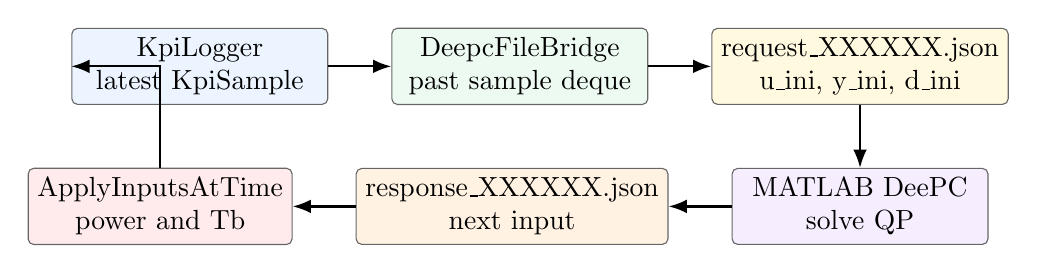
\begin{tikzpicture}[
  box/.style={rectangle, draw=black!60, rounded corners=2pt, align=center,
              minimum width=3.25cm, minimum height=0.82cm},
  arrow/.style={-Latex, thick},
  node distance=0.8cm
]
\node[box, fill=lightblue] (sample) {KpiLogger\\latest KpiSample};
\node[box, fill=lightgreen, right=of sample] (history) {DeepcFileBridge\\past sample deque};
\node[box, fill=lightyellow, right=of history] (request) {request\_XXXXXX.json\\u\_ini, y\_ini, d\_ini};
\node[box, fill=lightpurple, below=of request] (matlab) {MATLAB DeePC\\solve QP};
\node[box, fill=lightorange, left=of matlab] (response) {response\_XXXXXX.json\\next input};
\node[box, fill=lightred, left=of response] (apply) {ApplyInputsAtTime\\power and Tb};
\draw[arrow] (sample) -- (history);
\draw[arrow] (history) -- (request);
\draw[arrow] (request) -- (matlab);
\draw[arrow] (matlab) -- (response);
\draw[arrow] (response) -- (apply);
\draw[arrow] (apply) |- (sample);
\end{tikzpicture}
\end{center}

\subsection{\code{DeepcFileBridge} Methods}

\begin{center}
\begin{longtable}{L{0.30\linewidth}L{0.60\linewidth}}
\toprule
Member variable & Meaning \\
\midrule
\endhead
\code{m_bridgeDir}, \code{m_requestDir}, \code{m_responseDir} &
Base bridge directory and the two subdirectories used for request and response
JSON files. \\
\code{m_pastHorizon}, \code{m_futureHorizon} &
Number of past samples sent to MATLAB and number of future samples optimized by
MATLAB. \\
\code{m_timeoutS} &
Wall-clock timeout used while ns-3 waits for a response JSON file. \\
\code{m_samples} &
Deque of recent \code{KpiSample} values.  It is limited to
\code{m_pastHorizon}. \\
\code{m_hasLastPushedSample}, \code{m_lastPushedSampleTimeS} &
Bookkeeping used to avoid pushing the same KPI sample more than once. \\
\code{m_appliedOut} &
CSV stream for applied controls and response metadata. \\
\code{m_timingOut} &
CSV stream for wait times and MATLAB solve times. \\
\bottomrule
\end{longtable}
\end{center}

\begin{center}
\begin{longtable}{L{0.25\linewidth}L{0.27\linewidth}L{0.38\linewidth}}
\toprule
Method & Inputs and outputs & Function behavior \\
\midrule
\endhead
\code{Configure(bridgeDir,pastHorizon,futureHorizon,timeoutS)} &
Inputs: directory, horizons, timeout. &
Creates \code{requests} and \code{responses} directories, opens
\code{applied_controls.csv}, opens \code{controller_solve_times.csv}, and stores
bridge settings. \\
\code{PushSample(sample)} &
Input: \code{KpiSample}.  Output: bool. &
Adds a newer KPI sample to the history deque and keeps only the latest
\code{pastHorizon} samples.  Returns false if the sample was already pushed. \\
\code{Ready()} &
Output: bool. &
Returns true when the bridge has enough past samples to form a DeePC request. \\
\code{HistorySize()} &
Output: number of stored samples. &
Used for status printing. \\
\code{PastHorizon()} &
Output: configured past horizon. &
Used for status printing. \\
\code{HasHistory()} &
Output: bool. &
Indicates whether any KPI sample has been pushed. \\
\code{LatestSample()} &
Output: most recent \code{KpiSample}. &
Used for status printing and bridge logs. \\
\code{RequestControl(step,timeS,previousU)} &
Inputs: control step, current time, previous input.  Output: next
\code{InputCommand}. &
Writes a request JSON file, waits until the matching response JSON exists,
extracts \code{tx_power_dbm} and \code{beacon_interval_s}, logs timing and
applied controls, and returns the command. \\
\code{BuildStepPath(dir,prefix,step)} &
Inputs: directory, filename prefix, step.  Output: file path. &
Builds names such as \code{request_000004.json}. \\
\code{BuildUIni()} &
Output: vector of doubles. &
Flattens past sample inputs in time order as
\code{[p_0,Tb_0,p_1,Tb_1,...]}. \\
\code{BuildYIni()} &
Output: vector of doubles. &
Flattens past outputs as \code{[PRR,PIR,CBR]} for each stored sample. \\
\code{BuildDIni()} &
Output: vector of doubles. &
Flattens past context variables for each stored sample. \\
\code{BuildDFuture()} &
Output: vector of doubles. &
Repeats the latest context vector for each future horizon step. \\
\code{AppendContext(values,s)} &
Input: vector and sample. &
Appends active count, density, neighbor counts, and sensing exclusion ratio. \\
\code{WriteRequest(requestPath,step,timeS,previousU)} &
Inputs: path, step, time, previous input. &
Writes the full JSON request through a temporary file and then renames it
atomically. \\
\bottomrule
\end{longtable}
\end{center}

\subsection{\code{RunDeepcBridgeStep()}}

\code{RunDeepcBridgeStep()} is a scheduled simulator function rather than a class
method.  Each tick:

\begin{enumerate}
  \item reads the latest KPI sample from \code{KpiLogger};
  \item pushes it into the bridge history if it is new and inside the evaluation
  interval;
  \item prints bridge status;
  \item if enough history is available, writes a request and waits for MATLAB;
  \item applies the returned input to the CAM apps and NR UE PHYs;
  \item schedules the next bridge tick.
\end{enumerate}

Important control-mode rule:

\begin{lstlisting}[style=textstyle]
enableDeepcBridge=true requires useInputSchedule=false
\end{lstlisting}

The program aborts if both the PRBS schedule and the DeePC bridge are enabled,
because both would try to control transmit power and beacon interval.

\section{Main Output Files}

\begin{center}
\begin{longtable}{L{0.34\linewidth}L{0.56\linewidth}}
\toprule
Output & Contents \\
\midrule
\endhead
\code{kpi_timeseries_deepc_copy_run01.csv} &
Main time series:
\code{time_s}, \code{tx_power_dbm}, \code{beacon_interval_s},
\code{active_vehicle_count_core}, \code{density_veh_per_km_core},
\code{mean_neighbors_150m}, \code{mean_neighbors_300m},
\code{prr_awareness}, \code{pir_s}, \code{cbr},
\code{sensing_exclusion_ratio}. \\
\code{cbr_timeseries_deepc_copy_run01.csv} &
CBR data from \code{CbrLogger}. \\
\code{*_tx_packet_log.csv} &
One row per accepted transmission, including TX position and eligible receiver
counts by distance bin. \\
\code{*_rx_packet_log.csv} &
One row per accepted reception, including TX/RX node IDs, distance at TX time,
distance at RX time, PIR, and delay. \\
\code{*_metadata.json} &
Experiment settings, KPI definitions, radio configuration, CAM generation rule,
and dataset column definitions. \\
\code{bridge/requests/request_XXXXXX.json} &
Closed-loop DeePC requests written by ns-3. \\
\code{bridge/responses/response_XXXXXX.json} &
Closed-loop DeePC responses written by MATLAB. \\
\code{bridge/applied_controls.csv} &
Control values applied by ns-3 and response success/timing fields. \\
\code{bridge/controller_solve_times.csv} &
Wait time and solver time per DeePC bridge step. \\
\bottomrule
\end{longtable}
\end{center}

\section{MATLAB DeePC Controller}

\subsection{MATLAB Role}

\code{matlab_deepc_file_controller.m} is a file-watching controller.  It does not
run ns-3.  Instead, it waits for ns-3 to write request JSON files, solves a DeePC
optimization using pre-exported Hankel matrices, and writes response JSON files.

\subsection{MATLAB Parameters}

\begin{center}
\begin{longtable}{L{0.28\linewidth}L{0.18\linewidth}L{0.44\linewidth}}
\toprule
Parameter & Default & Meaning \\
\midrule
\endhead
\code{BridgeDir} &
\code{data/output/deepc_matlab_bridge_run01/bridge} &
Bridge directory containing \code{requests} and \code{responses}. \\
\code{DataMat} &
\code{data/output/deepc_open_loop_250veh/matlab_deepc_data.mat} &
MATLAB file containing normalized Hankel matrices and scaling data. \\
\code{YalmipDir} &
empty &
Optional path added recursively to MATLAB path. \\
\code{Solver} &
\code{quadprog} &
YALMIP solver name. \\
\code{PollSeconds} &
\code{0.05} &
Pause between directory scans when no request is found. \\
\code{IdleTimeoutSeconds} &
\code{0} &
If positive, exit after this many inactive seconds. \\
\code{MaxSteps} &
\code{0} &
If positive, exit after this many solved requests. \\
\code{MaxHankelCols} &
\code{300} &
Limits optimization size by selecting the closest Hankel columns to current
history. \\
\code{TargetPrr}, \code{TargetPir}, \code{TargetCbr} &
\code{0.95}, \code{0.10}, \code{0.35} &
Reference output trajectory. \\
\code{MinPowerDbm}, \code{MaxPowerDbm} &
\code{10.0}, \code{23.0} &
Bounds on transmit power. \\
\code{MinBeaconIntervalS}, \code{MaxBeaconIntervalS} &
\code{0.05}, \code{0.50} &
Bounds on beacon interval. \\
\code{WeightPrr}, \code{WeightPir}, \code{WeightCbr} &
\code{40.0}, \code{3.0}, \code{8.0} &
Output tracking weights. \\
\code{WeightPower}, \code{WeightBeaconInterval} &
\code{0.002}, \code{0.5} &
Input magnitude weights. \\
\code{LambdaY}, \code{LambdaG} &
\code{1.0e-3}, \code{1.0e-3} &
Regularization on future output and DeePC coefficient vector. \\
\bottomrule
\end{longtable}
\end{center}

\subsection{MATLAB Function-by-Function Explanation}

\begin{center}
\begin{tabular}{L{0.22\linewidth}L{0.68\linewidth}}
\toprule
MATLAB variable & Meaning \\
\midrule
\code{cfg} &
Parsed controller configuration from \code{inputParser}. \\
\code{data} &
Loaded MAT-file struct containing Hankel matrices, scaler vectors, horizons, and
column names. \\
\code{req} &
One decoded ns-3 request JSON. \\
\code{H} &
Sliced Hankel block struct for the request horizon. \\
\code{g} &
YALMIP DeePC trajectory-combination decision variable. \\
\code{uFuture}, \code{yFuture} &
YALMIP decision variables for future input and predicted output trajectories. \\
\code{diagnostics} &
YALMIP solver result; \code{diagnostics.problem == 0} means success. \\
\code{payload} &
Response struct written to JSON for ns-3. \\
\bottomrule
\end{tabular}
\end{center}

\begin{center}
\begin{longtable}{L{0.25\linewidth}L{0.27\linewidth}L{0.38\linewidth}}
\toprule
Function & Inputs and outputs & Function behavior \\
\midrule
\endhead
\code{matlab_deepc_file_controller(varargin)} &
Input: name-value parameters.  Output: none. &
Parses configuration, optionally adds YALMIP to the MATLAB path, loads the
Hankel data MAT file, creates the response directory, and enters a loop watching
for \code{request_*.json}.  For each new request it calls \code{solve_request()}
and writes an atomic response JSON. \\
\code{solve_request(req,data,cfg)} &
Input: decoded request struct, loaded MAT data, configuration.  Output:
\code{sol} struct. &
Normalizes current history, prepares Hankel blocks, optionally selects a subset
of close Hankel columns, defines YALMIP decision variables, solves the classical
DeePC QP, denormalizes the first future input, clips it to physical bounds, and
returns the command. \\
\code{prepare_hankel_for_request(data,req,nu,ny,nd)} &
Input: exported Hankel data, requested horizons, dimensions.  Output: struct
\code{H}. &
Slices the exported normalized Hankel matrices so shorter smoke-test horizons
can be used even when the exported data has larger horizons. \\
\code{as_column(value)} &
Input: array-like value.  Output: double column vector. &
Ensures JSON arrays and MATLAB arrays are represented as column vectors. \\
\code{square_sum(x)} &
Input: vector or matrix.  Output: scalar. &
Computes \(\sum_i x_i^2\). \\
\code{normalize_blocks(values,meanValues,stdValues,blockSize)} &
Input: stacked physical values and per-channel scaler.  Output: normalized
stacked values. &
Applies the same mean/std normalization to each time block. \\
\code{denormalize_blocks(normValues,meanValues,stdValues,blockSize)} &
Input: normalized stacked values and scaler.  Output: physical values. &
Inverse of \code{normalize_blocks()}. \\
\code{response_path_for(responseDir,requestName)} &
Input: response directory and request filename.  Output: response path. &
Maps \code{request_000004.json} to \code{response_000004.json}. \\
\code{write_json_atomic(path,payload)} &
Input: response path and struct.  Output: none. &
Writes JSON to a temporary file, then moves it into place so ns-3 does not read
a partially written response. \\
\bottomrule
\end{longtable}
\end{center}

\subsection{Classical DeePC Optimization in MATLAB}

For each request, MATLAB uses a Hankel coefficient vector \(g\).  The current
implemented constraints are:

\[
U_p g = u_{\mathrm{ini}}, \qquad
Y_p g = y_{\mathrm{ini}},
\]

\[
U_f g = u_{\mathrm{future}}, \qquad
Y_f g = y_{\mathrm{future}}.
\]

The input and output bounds are:

\[
u_{\min} \leq u_{\mathrm{future}} \leq u_{\max},
\qquad
y_{\min} \leq y_{\mathrm{future}} \leq y_{\max}.
\]

The current objective is:

\[
\sum R \odot u_{\mathrm{future}}^2
+ \sum Q \odot (y_{\mathrm{future}} - y_{\mathrm{ref}})^2
+ \lambda_y \|y_{\mathrm{future}}\|_2^2
+ \lambda_g \|g\|_2^2.
\]

The first optimized input block is applied:

\[
u_{\mathrm{apply}} =
\begin{bmatrix}
\mathrm{tx\_power\_dbm}\\
\mathrm{beacon\_interval\_s}
\end{bmatrix}.
\]

\subsection{MATLAB Data Shapes}

With two inputs, three outputs, five context variables, past horizon \(T_{\mathrm{ini}}\),
future horizon \(N\), and \(M\) Hankel columns:

\begin{center}
\begin{tabular}{L{0.16\linewidth}L{0.24\linewidth}L{0.50\linewidth}}
\toprule
Matrix/vector & Shape & Meaning \\
\midrule
\code{Up} & \((2T_{\mathrm{ini}}) \times M\) &
Past input Hankel block. \\
\code{Uf} & \((2N) \times M\) &
Future input Hankel block. \\
\code{Yp} & \((3T_{\mathrm{ini}}) \times M\) &
Past output Hankel block. \\
\code{Yf} & \((3N) \times M\) &
Future output Hankel block. \\
\code{Dp} & \((5T_{\mathrm{ini}}) \times M\) &
Past context Hankel block.  Loaded and sliced by MATLAB. \\
\code{Df} & \((5N) \times M\) &
Future context Hankel block.  Loaded and sliced by MATLAB. \\
\code{g} & \(M \times 1\) or selected columns \(\times 1\) &
DeePC trajectory-combination variable. \\
\code{uFuture} & \(2N \times 1\) &
Future control sequence optimized by DeePC. \\
\code{yFuture} & \(3N \times 1\) &
Future output sequence predicted by DeePC. \\
\bottomrule
\end{tabular}
\end{center}

\section{How the C++ and MATLAB Files Work Together}

\begin{enumerate}
  \item Start the MATLAB controller with the same \code{BridgeDir} that ns-3 will
  use.
  \item Run ns-3 with \code{--enableDeepcBridge=true --useInputSchedule=false}.
  \item ns-3 waits until enough KPI samples exist.
  \item ns-3 writes \code{bridge/requests/request_XXXXXX.json}.
  \item MATLAB reads the request and solves DeePC.
  \item MATLAB writes \code{bridge/responses/response_XXXXXX.json}.
  \item ns-3 reads the response, applies transmit power and beacon interval, and
  logs the action.
  \item The process repeats every bridge control interval when a new KPI sample is
  available.
\end{enumerate}

Example ns-3 command shape:

\begin{lstlisting}[style=textstyle]
./ns3 run "nr_v2x_ngsim_deepc_copy \
  --enableDeepcBridge=true \
  --useInputSchedule=false \
  --deepcBridgeDir=data/output/deepc_matlab_bridge_run01/bridge \
  --kpiCsv=data/output/deepc_matlab_bridge_run01/kpi_timeseries.csv \
  --cbrCsv=data/output/deepc_matlab_bridge_run01/cbr_timeseries.csv"
\end{lstlisting}

Example MATLAB command shape:

\begin{lstlisting}[style=matlabstyle]
matlab_deepc_file_controller( ...
    'BridgeDir', 'data/output/deepc_matlab_bridge_run01/bridge', ...
    'DataMat', 'data/output/deepc_open_loop_250veh/matlab_deepc_data.mat', ...
    'Solver', 'quadprog')
\end{lstlisting}

\section{Review Notes for Professor Feedback}

The following points are not errors by themselves, but they are useful review
targets.

\begin{enumerate}
  \item \textbf{KPI sample interval}: \code{sampleTimeS} is currently initialized
  to \code{1}, while the nearby comment says ``100 ms KPI sampling interval.''  If
  the intended sample time is 100 ms, the value should be \code{0.1}.
  The metadata text also describes 0.1 s KPI/CBR alignment, so the numeric
  default, comments, and metadata should be made consistent.
  \item \textbf{Beacon interval lower bound mismatch}: C++ \code{SetBeaconInterval()}
  uses \code{max(0.1,tb)}, while MATLAB allows \code{MinBeaconIntervalS = 0.05}.
  Commands below 0.1 s will be clipped by the C++ CAM app behavior.
  \item \textbf{Context variables in MATLAB}: ns-3 sends \code{d_ini} and
  \code{d_future}, and MATLAB slices \code{Dp} and \code{Df}, but the current QP
  does not constrain or penalize context matching.  If context-aware DeePC is the
  research objective, add constraints or slack terms involving \code{Dp*g} and
  \code{Df*g}.
  \item \textbf{Unused MATLAB weights}: parameters such as \code{WeightDeltaPower},
  \code{WeightDeltaBeaconInterval}, \code{LambdaIniU}, \code{LambdaIniY},
  \code{LambdaIniD}, and \code{LambdaFutureD} are parsed but not used in the
  current optimization.
  \item \textbf{Input reference parameters}: \code{TargetPowerDbm} and
  \code{TargetBeaconIntervalS} are parsed by MATLAB but the objective currently
  penalizes input magnitude, not deviation from those target inputs.
  \item \textbf{CAM size setting}: \code{maxCamSizeBytes} is passed into
  \code{CamApplication::Setup()} and stored, but the current code does not use it
  to truncate or validate encoded CAM packet size.
  \item \textbf{Manual JSON parsing in C++}: response parsing uses simple
  key-based extraction helpers.  This is acceptable for the small controlled
  schema, but a JSON library would be more robust if the schema grows.
\end{enumerate}

\section{One-Page Mental Model}

\begin{lstlisting}[style=textstyle]
Mobility CSV
  -> MobilityRow records
  -> g_mobilityByVehicle
  -> ns-3 vehicle nodes
  -> WaypointMobilityModel
  -> moving vehicles

Open-loop control
  -> InputCommand records from prbs_schedule.csv
  -> Simulator::Schedule input updates
  -> ApplyInputsAtTime changes power and beacon interval

Closed-loop control
  -> KpiLogger produces KpiSample rows
  -> DeepcFileBridge stores past samples
  -> request_XXXXXX.json sent to MATLAB
  -> MATLAB solves classical DeePC
  -> response_XXXXXX.json returns next input
  -> ApplyInputsAtTime changes power and beacon interval

Packet measurement
  -> CAM generated by CABasicService
  -> KpiPacketTag added at transmit callback
  -> LogTx records eligible receiver opportunities
  -> NR sidelink delivers or drops packet
  -> ReceiveCam handles successful receptions
  -> LogRx records successful Tx/Rx/seq
  -> SampleAndWrite computes PRR, PIR, CBR, density, neighbors
\end{lstlisting}

\section{Suggested Reading Order}

\begin{enumerate}
  \item Read the data structures: \code{MobilityRow}, \code{InputCommand},
  \code{TxEvent}, \code{RxEvent}, and \code{KpiSample}.
  \item Read \code{LoadMobilityCsv()}, \code{InstallWaypointMobility()}, and the
  node-creation block in \code{main()}.
  \item Read \code{CamApplication::TagAndLogTx()} and
  \code{CamApplication::ReceiveCam()} to understand packet events.
  \item Read \code{KpiLogger::LogTx()}, \code{KpiLogger::LogRx()}, and
  \code{KpiLogger::SampleAndWrite()} to understand KPI definitions.
  \item Read \code{DeepcFileBridge} and \code{RunDeepcBridgeStep()} to understand
  the closed-loop connection.
  \item Read \code{matlab_deepc_file_controller.m}, especially
  \code{solve_request()}, to understand the controller optimization.
  \item Read the NR sidelink configuration in \code{main()} last, because it is
  ns-3 NR API-specific and less important for understanding the DeePC data flow.
\end{enumerate}

\end{document}
